%
%  Erik Olsen
%
\documentclass[12pt,fullpage]{article}
\usepackage{fullpage}                                        % use all of the page for text 
\usepackage{psfrag}                                          % LaTeX graphics tool
\usepackage{pslatex}                                         % avoids the default cmr font
\usepackage{graphicx}                                        % graphics package 
\usepackage{epsfig}                                          % figures
\usepackage{epsfig} 
\usepackage{hyperref}
\usepackage{color}

\begin{document}

\noindent
{\bf Standard power distribution}  (from \color{blue}\url{http://www.math.wm.edu/~leemis/chart/UDR/UDR.html}\color{black})

\noindent
The shorthand $X \sim {\rm power}(1,\beta)$ is used to indicate that the
random variable $X$ has the standard power distribution with shape parameter $\beta > 0$.
A standard power random variable $X$ with parameter $\beta$ has probability density function 
$$
f(x) = \beta \kern 0.04em x ^ {\kern 0.04em\beta - 1} \qquad \qquad 0 < x < 1.
$$
The probability density function with two different values of $\beta$ is illustrated below.
{\begin{figure}[h!]
\begin{center}
\psfrag{lab1}{$\beta = 0.5$}
\psfrag{lab2}{$\beta = 3$}
\psfrag{labx}{$x$}
\psfrag{labf}{$f(x)$}
\includegraphics[width=3.2in]{StandardpowerPlot.ps}
\end{center}
\end{figure}}\\
The cumulative distribution function on
the support of $X$ is
$$
F(x) = P(X \le x) = x ^ {\kern 0.04em\beta}  \qquad \qquad 0 <  x < 1.
$$
The survivor function on the support of $X$ is
$$
S(x) = P(X \ge x) = 1-x^{\kern 0.04em\beta} \qquad \qquad 0  < x < 1.
$$
The hazard function on the support of $X$ is
$$
h(x) = \frac{f(x)}{S(x)} = \frac{\beta x^{\kern 0.04em\beta-1}}{1-x^{\kern 0.04em \beta}} \qquad \qquad 0 < x < 1.
$$
The cumulative hazard function on the support of $X$ is
$$
H(x) = - \ln S(x) = - \ln(1 - x ^ {\kern 0.04em \beta}) \qquad \qquad 0 < x < 1.
$$
The inverse distribution function of $X$ is
$$
F ^ {-1}(u) = u ^ {1 / \beta} \qquad \qquad 0 < u < 1.
$$
The median of $X$ is
$$
\left(\frac{1}{2}\right) ^ {1 / \beta}.
$$
The population mean, variance, skewness, and kurtosis of $X$ are
$$
E[X] = \frac{\beta}{\beta + 1} \qquad \qquad 
V[X] = \frac{\beta}{(\beta+2)(\beta + 1)^2} \qquad \qquad 
$$
$$
E\left[ \left( \frac{X - \mu}{\sigma} \right) ^ {\kern -0.08em 3} \right]  = \frac{2 (1 - \beta) \sqrt{\beta + 2}}{(\beta + 3)\sqrt{\beta}} \qquad \qquad 
E\left[ \left( \frac{X - \mu}{\sigma} \right) ^ {\kern -0.08em 4} \right] = \frac{3 \left(3 \beta ^ 2 - \beta + 2\right)\left(\beta + 2\right)}{\beta(\beta + 3)(\beta + 4)}.
$$ \\
%For $X_1, \, X_2, \, \ldots , \, X_n$ mutually independent standard power($\lambda$) random variables,
%the maximum likelihood estimator for $\beta$ is
%$$
%\hat \beta = - \frac{n}{\sum_{i = 1} ^ n \ln(X_i)}.
%$$


%\newpage

\noindent
{\bf APPL verification:}
The APPL statements
\begin{verbatim}
assume(beta > 0);
X := [[x -> beta * x ^ (beta - 1)], [0, 1], ["Continuous", "PDF"]];
Mean(X);
Variance(X);
Skewness(X);
Kurtosis(X);
MGF(X);
\end{verbatim}
verify the population mean, variance, skewness, kurtosis, and moment generating function.
\end{document}
